\section{Introduction}

Molecular crystals are widely used in pharmaceuticals, agrochemicals, and organic electronics~\citep{beran2023frontiers}. Their properties depend strongly on molecular conformation and packing, and different polymorphs of the same chemical system can exhibit distinct solubility, stability, bioavailability, charge transport, and mechanical properties~\citep{price2014predicting,jin2025oxtal,gharakhanyan2025fastcsp}. Molecular crystal structure prediction (CSP) aims to predict possible crystal structures given the molecular components, accelerating drug development and functional materials design.

Molecular CSP generally involves two complementary stages: structure generation and structure ranking~\citep{hunnisett2024seventhranking,hunnisett2024seventhgeneration}. Traditional workflows generate candidate packings using random, quasi-random, or evolutionary search~\citep{li2018genarris,curtis2018gator}, then relax and rank them using computationally expensive energy calculations, often based on density functional theory~\citep{price2014predicting,reilly2016sixth,hunnisett2024seventhranking,hunnisett2024seventhgeneration}. FastCSP primarily accelerates structure ranking by using a machine-learning interatomic potential (MLIP) for structure relaxation and energy calculation, while obtaining initial candidates from a random structure generator~\citep{gharakhanyan2025fastcsp}.

Generative models offer a faster approach to structure generation by learning from experimentally observed crystal structures and concentrating a finite candidate budget on plausible packings. Despite recent progress~\citep{jin2025oxtal,zeng2026molcrystalflow,subramanian2026packflow,lo2026clari}, several gaps remain. Existing methods differ in the molecular information they require and the chemical systems they support, while evaluation protocols vary in candidate budgets and downstream processing, making generation and ranking performance difficult to compare directly. Moreover, the effects of key design choices in architecture, training, conditioning, inference, and scaling remain only partially understood.

In this work, we present \model{}, an all-atom generative model for molecular CSP that jointly predicts atomic coordinates and the unit cell from molecular graphs containing atom types, bond types, and formal charges. \model{} supports multi-component and organometallic crystals and explicitly models hydrogen atoms. A single model can also condition on additional structural information that is often available or readily derivable, such as molecular templates, stereochemical labels, and space-group information, allowing it to adapt to different levels of prior knowledge.

We also introduce a matched two-track evaluation that separates structure generation from structure ranking, following the CCDC CSP blind tests~\citep{hunnisett2024seventhranking,hunnisett2024seventhgeneration}. The generation track measures whether a fixed candidate set contains the experimental structure, without relaxation or energy-based ranking, thereby isolating generator coverage. The ranking track instead processes candidates from each generator through the same relaxation, filtering, deduplication, and lattice-energy ranking pipeline and measures whether the experimental form is ranked near the top. This separation enables direct comparison of generator quality and the downstream utility of generated candidates in practical CSP workflows.

Finally, we systematically study key design choices in architecture, training recipe, conditioning, inference, and scaling. We directly compare DiT with pair-bias attention~\citep{peebles2023scalable}, Pairformer~\citep{Abramson2024}, and Pairmixer~\citep{ouyangzhang2025triangle}, and ablate training choices such as time sampling, translation augmentation, and loss design. These studies show that cacheable pairwise reasoning substantially improves generation quality, careful training and sampling choices matter, and balanced scaling of pairwise and single representations preserves coverage at larger model sizes.

\begin{figure*}[!t]
  \centering
  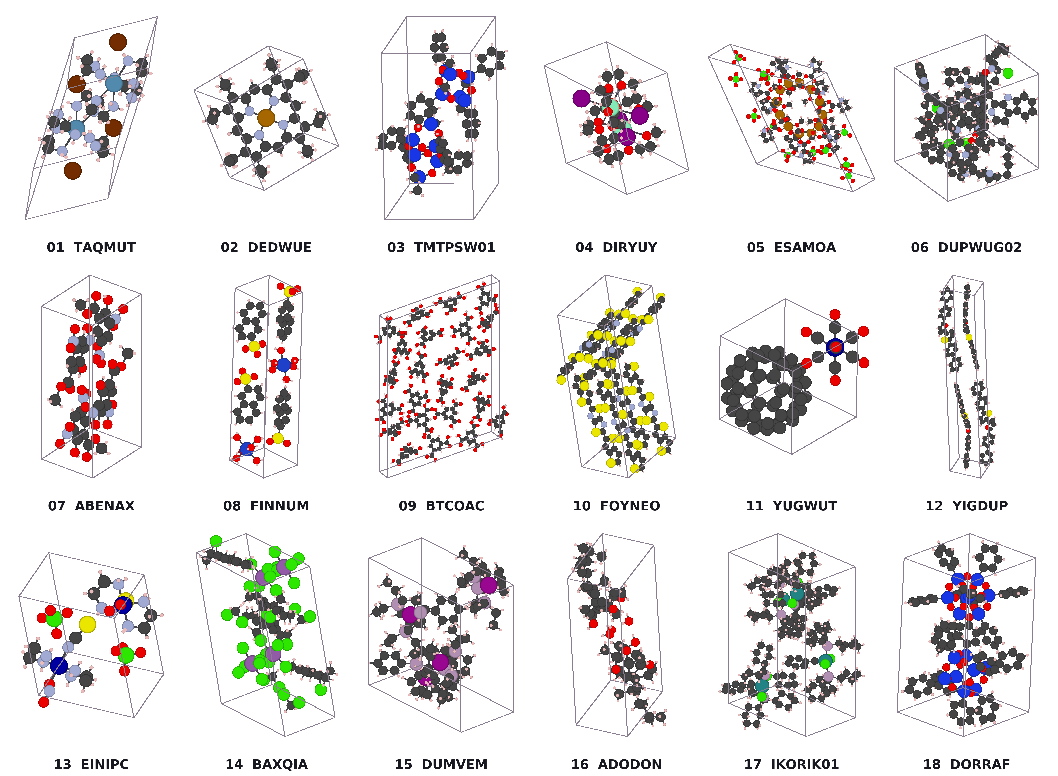
\includegraphics[width=\textwidth,height=0.82\textheight,keepaspectratio]{figures/generated/fig_strict_structure_examples.pdf}
  \caption{\textbf{Crystal structures predicted by \model{}.}
    Each example is a collision-free prediction from \model{}-L that matches all
    15 molecules of the experimental reference with
    $\mathrm{RMSD}_{15}<2\,\text{\AA}$. These 18 examples illustrate \model{}'s ability to generate diverse crystal structures across molecular sizes, compositions, packing motifs, and unit-cell geometries. Panel labels indicate the corresponding CSD refcodes.}
  \label{fig:strict-structure-examples}
\end{figure*}

For structure generation, across six benchmarks, \model{}-M or \model{}-L achieves the best coverage across candidate budgets and evaluation criteria, with up to a 77.6\% relative improvement over CLARI-H (\Cref{tab:benchmark_solc_main}). When combined with downstream relaxation and ranking, \model{} achieves higher recovery, faster convergence, and lower experimental-form ranks than CLARI-H on both the single-form and polymorph FastCSP benchmarks~\citep{gharakhanyan2025fastcsp}.

In summary, our contributions are:
\begin{itemize}
    \item \textbf{A flexible all-atom generative model for molecular CSP.}
    \model{} jointly generates atomic coordinates and unit cells for diverse molecular systems while supporting optional conditioning on molecular templates, stereochemistry, and space groups.
    \item \textbf{A matched evaluation of generation and ranking.}
    We separately measure finite-budget generator coverage and downstream performance under a common relaxation-and-ranking pipeline.
    \item \textbf{A systematic study of molecular CSP generative modeling.}
    We investigate architecture, training, conditioning, inference, and scaling under a common evaluation protocol and derive an evidence-backed design recipe.
\end{itemize}